\documentclass{article}
\usepackage{amsmath}
\usepackage{amsfonts}
\usepackage{tikz}
\usepackage{pgfplots}
\pgfplotsset{compat=1.16}

\begin{document}

\begin{figure}[h]
    \centering
    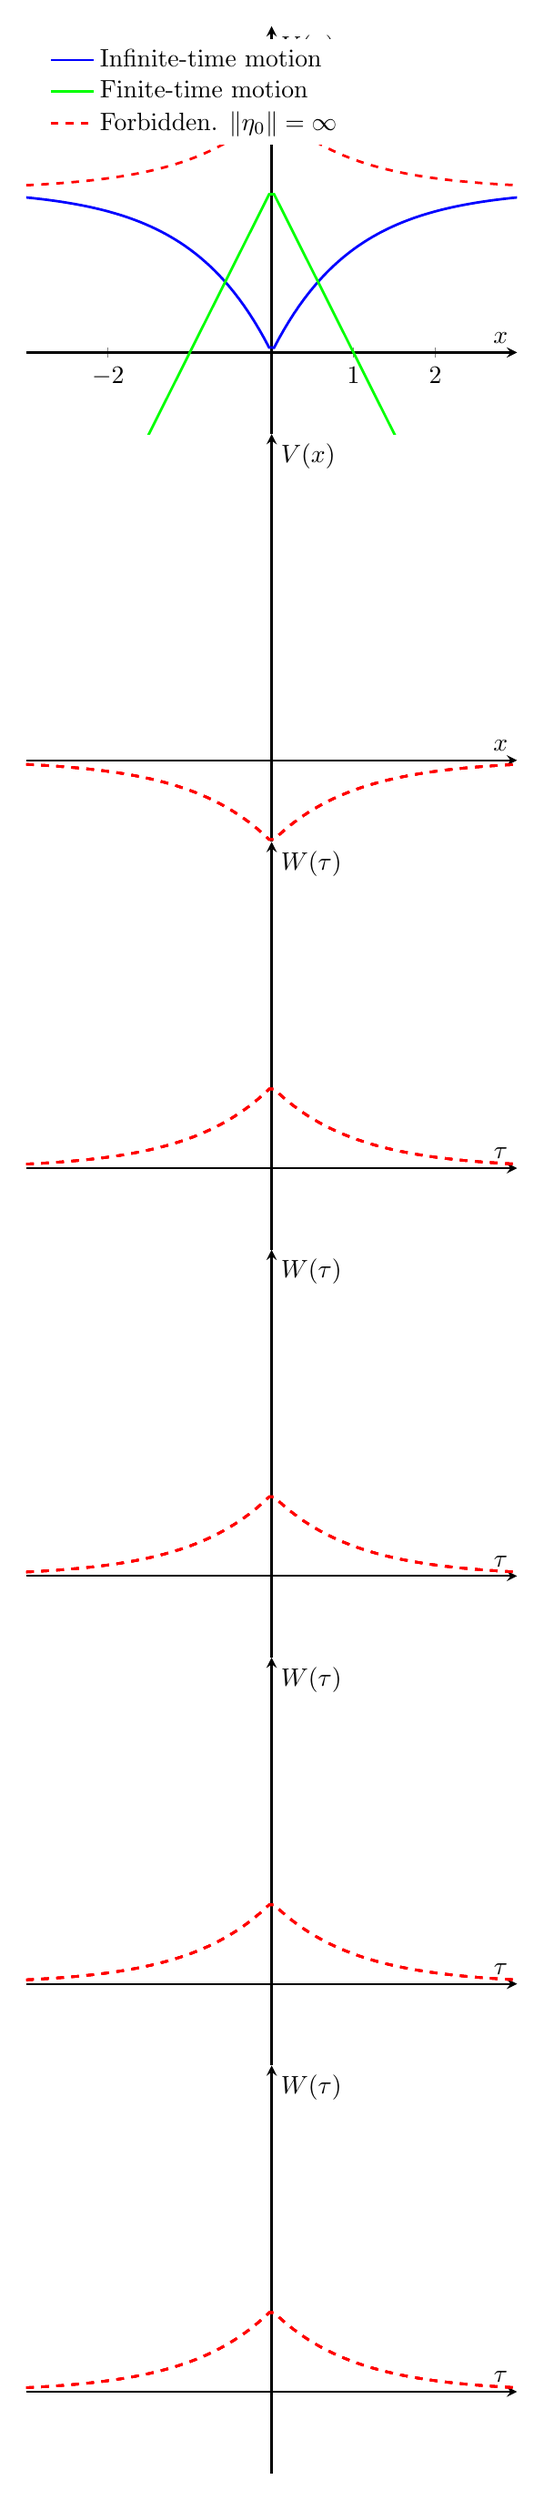
\begin{tikzpicture}
        \begin{axis}[
            axis lines=middle,
            xlabel=$x$,
            ylabel=$V(x)$,
            xmin=-3, xmax=3,
            ymin=-0.5, ymax=2,
            xtick={-2, 0, 1, 2},
            ytick=\empty,
            legend pos=north west,
            legend cell align=left,
            legend style={draw=none},
            domain=-3:3,
            samples=100,
            no markers,
            thick,
            every axis plot/.append style={line width=1pt},
            ]
            \addplot [blue] {1 - exp(-abs(x))};
            \addlegendentry{Infinite-time motion}
            \addplot [green] {1 - abs(x)};
            \addlegendentry{Finite-time motion}
            \addplot [red, dashed] {1 + 0.5*exp(-abs(x))};
            \addlegendentry{Forbidden. $\|\eta_0\| = \infty$}
        \end{axis}
        
        \begin{axis}[
            at={(current axis.south west)},
            anchor=north west,
            axis lines=middle,
            xlabel=$x$,
            ylabel=$V(x)$,
            xmin=-3, xmax=3,
            ymin=-0.5, ymax=2,
            xtick=\empty,
            ytick=\empty,
            domain=-3:3,
            samples=100,
            no markers,
            thick,
            every axis plot/.append style={line width=1pt},
            ]
            \addplot [red, dashed] {-1/2*exp(-abs(x))};
            \addplot [red, dashed] {-1/2*exp(-abs(x))};
            \addplot [red, dashed] {-1/2*exp(-abs(x))};
            \addplot [red, dashed] {-1/2*exp(-abs(x))};
        \end{axis}
        
        \begin{axis}[
            at={(current axis.south west)},
            anchor=north west,
            axis lines=middle,
            xlabel=$\tau$,
            ylabel=$W(\tau)$,
            xmin=-3, xmax=3,
            ymin=-0.5, ymax=2,
            xtick=\empty,
            ytick=\empty,
            domain=-3:3,
            samples=100,
            no markers,
            thick,
            every axis plot/.append style={line width=1pt},
            ]
            \addplot [red, dashed] {1/2*exp(-abs(x))};
            \addplot [red, dashed] {1/2*exp(-abs(x))};
            \addplot [red, dashed] {1/2*exp(-abs(x))};
            \addplot [red, dashed] {1/2*exp(-abs(x))};
        \end{axis}
        
        \begin{axis}[
            at={(current axis.south west)},
            anchor=north west,
            axis lines=middle,
            xlabel=$\tau$,
            ylabel=$W(\tau)$,
            xmin=-3, xmax=3,
            ymin=-0.5, ymax=2,
            xtick=\empty,
            ytick=\empty,
            domain=-3:3,
            samples=100,
            no markers,
            thick,
            every axis plot/.append style={line width=1pt},
            ]
            \addplot [red, dashed] {1/2*exp(-abs(x))};
            \addplot [red, dashed] {1/2*exp(-abs(x))};
            \addplot [red, dashed] {1/2*exp(-abs(x))};
            \addplot [red, dashed] {1/2*exp(-abs(x))};
        \end{axis}
        
        \begin{axis}[
            at={(current axis.south west)},
            anchor=north west,
            axis lines=middle,
            xlabel=$\tau$,
            ylabel=$W(\tau)$,
            xmin=-3, xmax=3,
            ymin=-0.5, ymax=2,
            xtick=\empty,
            ytick=\empty,
            domain=-3:3,
            samples=100,
            no markers,
            thick,
            every axis plot/.append style={line width=1pt},
            ]
            \addplot [red, dashed] {1/2*exp(-abs(x))};
            \addplot [red, dashed] {1/2*exp(-abs(x))};
            \addplot [red, dashed] {1/2*exp(-abs(x))};
            \addplot [red, dashed] {1/2*exp(-abs(x))};
        \end{axis}
        
        \begin{axis}[
            at={(current axis.south west)},
            anchor=north west,
            axis lines=middle,
            xlabel=$\tau$,
            ylabel=$W(\tau)$,
            xmin=-3, xmax=3,
            ymin=-0.5, ymax=2,
            xtick=\empty,
            ytick=\empty,
            domain=-3:3,
            samples=100,
            no markers,
            thick,
            every axis plot/.append style={line width=1pt},
            ]
            \addplot [red, dashed] {1/2*exp(-abs(x))};
            \addplot [red, dashed] {1/2*exp(-abs(x))};
            \addplot [red, dashed] {1/2*exp(-abs(x))};
            \addplot [red, dashed] {1/2*exp(-abs(x))};
        \end{axis}
    \end{tikzpicture}
    \caption{Typical shapes of $V(x)$ for various regions of $\gamma$ together with the corresponding $W(\tau)$. Arrows indicate directions to the turning points. Dotted lines show the regions where the behavior of the functions can be modified by higher-order corrections to (\ref{eq:pot_as}).}
    \label{fig:shapes}
\end{figure}

\end{document}